\documentclass[12pt]{article}
\usepackage[utf8]{inputenc}
\usepackage{lmodern}
\usepackage[left=1.5cm, right=1.5cm, top=1.5cm]{geometry}
\usepackage[utf8]{inputenc}
\usepackage[T1]{fontenc}
\usepackage{microtype}
\usepackage[dvips]{graphicx}
\usepackage{xcolor}
\usepackage{times}
\usepackage{gensymb}
\usepackage{paralist}
\usepackage{cite}
\usepackage{amsmath, amssymb, amsthm}
\usepackage{siunitx}
\usepackage{underscore}
\usepackage{url}
\usepackage{float}
\usepackage{booktabs}
\usepackage{enumitem}
% if you want simple numeric cites
\usepackage{cite}
\usepackage[authoryear]{natbib}  % in your preamble

% or, for author–year and more flexible commands (\citet, \citep, etc.)
\usepackage{natbib}
% then in the body use \citet{bollmann19} or \citep{bollmann19}
% in your preamble

\usepackage[parfill]{parskip}
%\usepackage{cite} % takes care of citations
\usepackage[final]{hyperref} % adds hyper links inside the generated pdf file
\hypersetup{
	colorlinks=true,       % false: boxed links; true: colored links
	linkcolor=blue,        % color of internal links
	citecolor=blue,        % color of links to bibliography
	filecolor=magenta,     % color of file links
	urlcolor=blue         
}
\usepackage{minted}
\large
\title{BREE Research paper}
\begin{document}
\begin{titlepage}
	\begin{center}
    \line(1,0){300}\\
    [0.65cm]
	\huge{\bfseries Concordance Mapping of U.S. Tariffs Over 250 Years}\\
	\line(1,0){300}\\
	\textsc{\Large Samir Kadariya}\\
	% \textsc{\LARGE \today}\\
	[5.5cm]     
	\end{center}

\end{titlepage}

\tableofcontents

\newpage

\section{Abstract}
Modern economic analyses often require linking centuries-old U.S. tariff schedules--written in archaic prose and coded until multiple, now-obsolete systems--to today's eight-digit Harmonized System (HS). We present the first fully automated concordance that threads every tariff line from the 1789 Tariff Act through four major coding overhauls into the 2023 HS vocabulary. The pipeline "walks" backwards one calendar year at a time: each description is (i) modernized with a GPT-4 prompt, (ii) embedded with the sentence-transformer MPNet, and (iii) matched to its nearest neighbor in the previous year using a composite similarity score. When that score dips below a specified threshold, we first apply a hierarchical HS fallback--matching at the 2-, 4-, or 6- digit level appropriate to the historical regime--before any remaining low-confidence records trigger a Selenium-based query to the U.S. Census HS-Classifier, with GPT selecting among the most probable codes the website outputs. On three public schedules--1789 (free text), 1963 (TSUS-8) and 1989 (HS-8)--the method attains a $65\%$, $75\%$, and $90\%$ percent similarity score, respectively.  The resulting open-source concordance and Python package let researchers map any historical description to a ranked list of 2023 HS codes with confidence scores, enabling consistent long-run trade analyses without manual recoding. 

\section{Introduction}


U.S. trade policy has evolved dramatically over the last 250 years, and its history is documented through a diverse array of tariff schedules. These records capture shifts in economic priorities, global market changes, and changes in political and technological contexts. In the real world, understanding these changes is important for economic historians, policymakers, and researchers who analyze long-term trends in trade practices. Tariffs--being one of the primary measures of trade regulation--offer insights into how governments respond to economic pressures and how these responses influenced the market over time. 

However, studying these tariff documents is hindered by three barriers: archaic language, inconsistent formatting, and obsolete coding schemes. These elements are misaligned with modern classification standards, like the Harmonized System (H.S.). Figure 1 below illustrates the historical evolution of U.S. tariff coding systems from 1789 onward.

This misalignment makes it challenging for researchers to draw meaningful conclusions between historical and modern data. Without a standardized basis for analysis, it is difficult to assess accurately the evolution of trade policy or the long-term impact of past economic decisions. Recent advances in natural language processing (NLP) and machine learning provide promising ways for addressing these challenges. 

\begin{figure}[H]
    \centering
    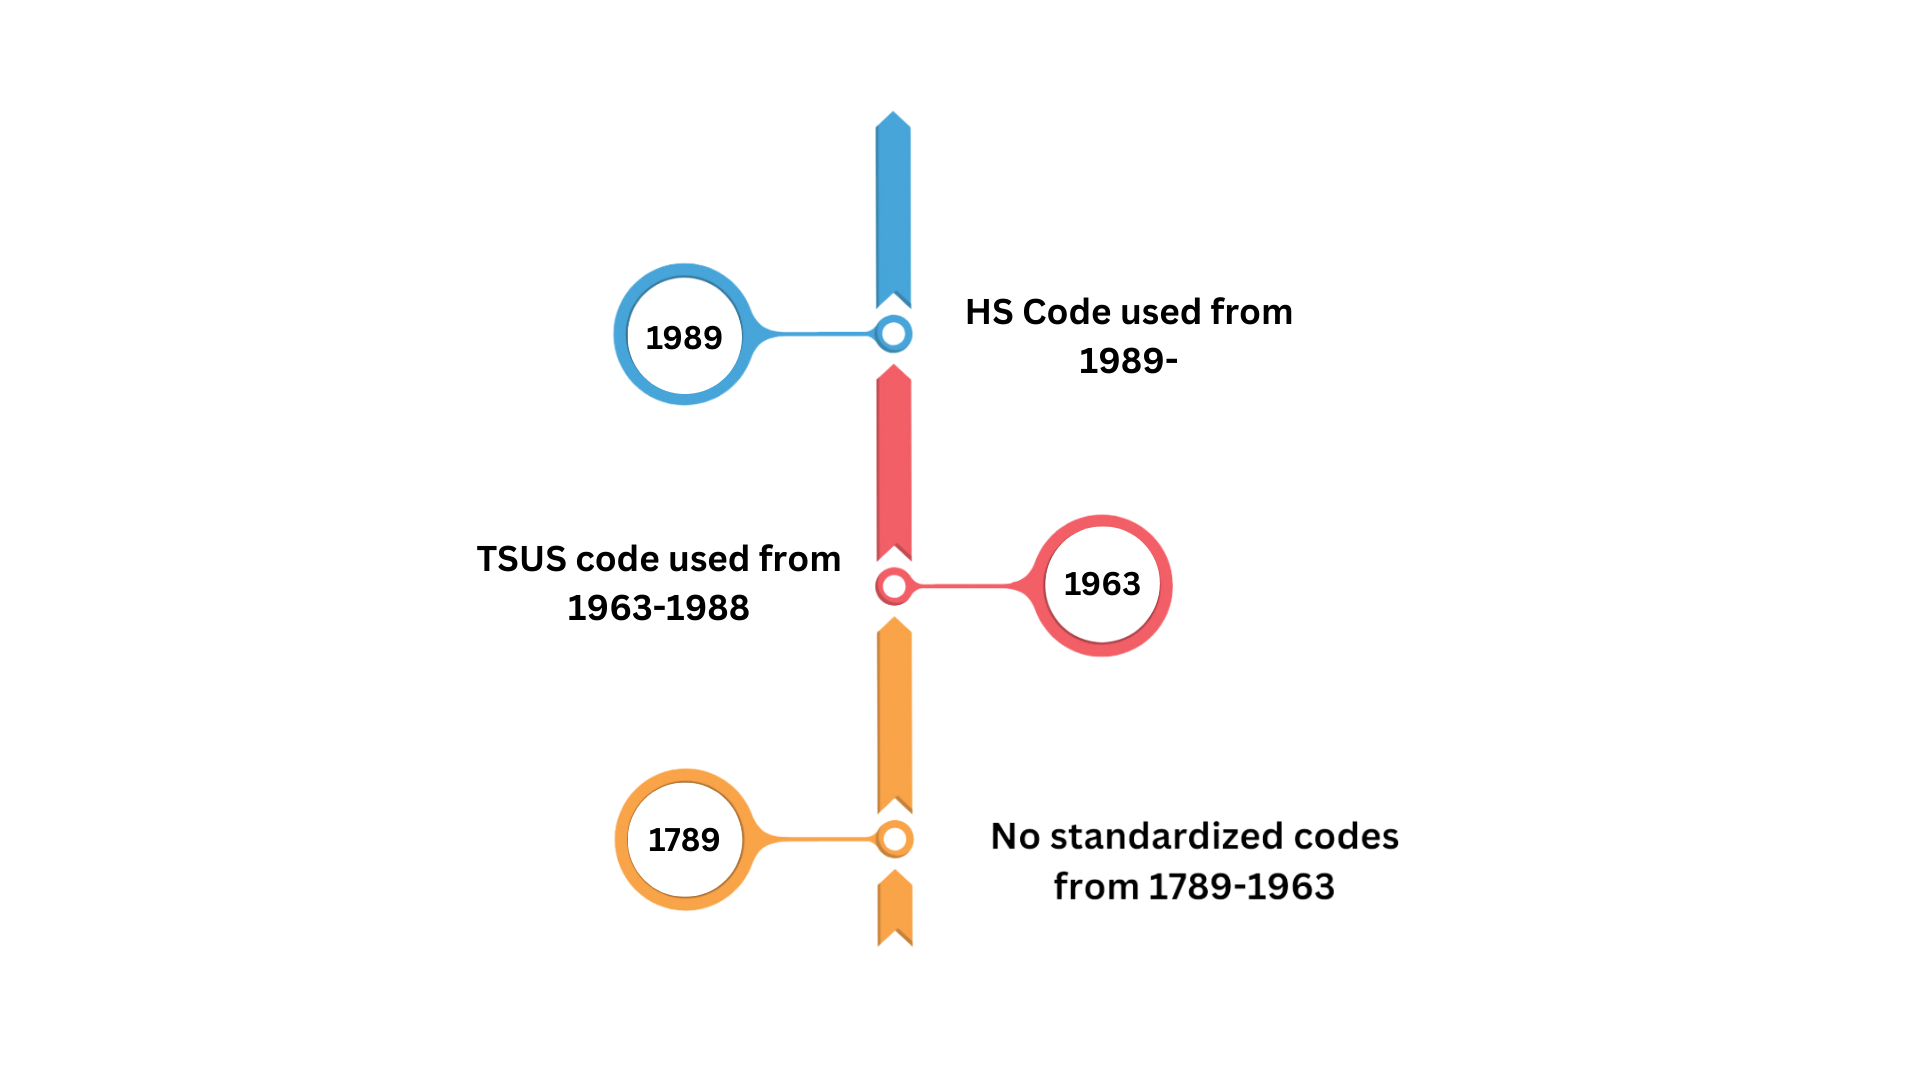
\includegraphics[width=0.69\linewidth]{tariff-evolution.png}
    \caption{Evolution of U.S. commodity-coding systems. Before 1963 tariff acts listed goods without a standardized numeric scheme; the TSUS (Tariff Schedules of the United States) was introduced in 1963 and remained in force until 1988; in 1989, the United States adopted the Harmonized System (H.S.), which has been revised roughly every five years since.}
    \label{fig:enter-label}
\end{figure}


The central research problem addressed by this paper is translating centuries-old, ambiguous tariff descriptions into modern H.S. codes. Historical records are full of region-specific terminologies and inconsistent coding practices. 
They lack the consistency for direct comparison with modern data, which is important for developing a narrative of how trade policy has evolved. 

Prior work has developed end-to-end ML pipelines for aligning product descriptions across domains, but those models assume clean, HS-like metadata that nineteenth-century tariffs lack. Other efforts have advanced semantic-similarity detection with transformer-based Siamese architectures and large-scale historical text-normalization to correct orthographic drift, yet they either focus on modern corpora or ignore successive changes in coding schemes. A unified method that bridges both linguistic drift and evolving commodity codes across centuries of tariff data remains absent.


By addressing both the language and structural challenges of tariff descriptions, our work fills a critical gap in the literature and offers a new framework for integrating historical tariff data into modern trade policy analysis. To our knowledge, no one has combined these different areas of NLP and text modernization to build a century-spanning, machine-generated concordance that is text-aware. 
\newline

This paper makes three contributions:

\begin{itemize}
    \item \textbf{Iterative back-mapping}. We introduce an NLP pipeline that "walks" backward one year at a time--from 2023 to 1789--modernizing each tariff description as necessary using GPT, embedding it with MPNet, and then matching it to the closest item in the previous years' tariff schedule. These short, adjacent steps preserve continuity through each H.S. revision, avoiding the semantic cliff that occurs when jumping directly from a previous year (like 1789) to 2023.
    \item \textbf{Hybrid Verification}. For the small fraction for lines whose similarity falls below some empirical threshold (for example, below 0.5), we invoke an automated Selenium and GPT wrapper that queries the U.S. Census "H.S. Classifier" website. This life site forces the algorithm to reconcile ambiguous descriptions with the most similar and specific H.S. code in force today. 

    \item \textbf{Open-source query package}. Alongside the full machine-readable concordance, we will release a Python package that lets users supply any tariff description and receive (i) the best-matching 2023 H.S. code (up to the most appropriate and specific digit), (ii) associated modern description, and (iii) the similarity score plus the confidence flag. The package ships with pre-computed embeddings and fallback website-verification routine, so a single call returns a ranked list of candidate H.S. codes quickly, enabling researchers to integrate historical or ad-hoc product lines directly into current H.S.-based datasets. 
\end{itemize}



We expect that this integrated approach will yield a significant improvement in the accuracy and consistency of H.S. code predictions for historical tariff data. The use of NLP techniques should enable the system to capture complex semantic information from the historical documents, while the real-time verification module is expected to minimize misclassification by comparing predictions from the NLP model to the one form the U.S. census website. Key metrics will include prediction accuracy (quantified by F1 score) and cosine similarity scores, which provide a measure of confidence in the semantic matching process. 

The remainder of the article is organised as follows.
Section 2 details the dual-pipeline methodology, including data pre-processing, embedding generation, year-to-year chaining, and the fallback website module. Section 3 reports similarity trends, H.S.-hierarchy retention rates, and case studies of low-confidence mappings. Section 4 discusses limitations and future work.

By demonstrating that a largely automated system can track tariff descriptions through three decades and four major H.S. overhauls, we provide a practical foundation for consistent historical trade analysis—without the years of manual concordance work previously required.
\newpage

\section{Related Work}

\subsubsection*{Product Description Matching}  
Prior research in product data alignment has tackled challenges similar to our tariff‐mapping problem. \citeauthor{desantana23} present an end‐to‐end machine‐learning pipeline for matching contemporary e-commerce product listings across different retailers. Their system leverages structured product metadata (akin to our H.S.\ category codes) and text features to align items that are essentially the same product \cite{desantana23}. This approach achieves high accuracy in modern, well‐formatted datasets, but it assumes the availability of clean, standardized descriptors—a condition that breaks down for nineteenth‐century tariffs and older records. Similarly, \citeauthor{viji22} propose a hybrid semantic similarity model combining a fine‐tuned BERT encoder with a Siamese Bi-LSTM network to improve the detection of matching or duplicate product descriptions by capturing nuanced semantic relationships \cite{viji22}. While this method performs strongly on benchmark datasets (e.g., modern product reviews or Q\&A pairs), it has been evaluated only on contemporary language and struggles with the domain gap presented by historical text: archaic vocabulary, inconsistent spelling, and an absence of structured categorization. In contrast, our approach does not assume any standardized fields in the input. By iteratively linking items year by year, we tackle both description matching and code alignment together, avoiding the “semantic cliff” that a single‐step matching baseline would encounter when bridging centuries of terminology.

\subsubsection*{Historical Text Normalization}  
A separate line of research has addressed linguistic drift in long‐term text archives. \citeauthor{bollmann19} conduct a large‐scale comparison of historical text normalization techniques, evaluating rule‐based and neural methods to map archaic spelling variants to modern forms \cite{bollmann19}. Their findings highlight the importance of robust text normalization for improving NLP on historical documents. However, these studies focus chiefly on orthographic and lexical changes, independent of any evolving classification system. They do not consider the concurrent evolution of domain‐specific labels, such as tariff item codes that shift over time. Our work builds upon these insights—employing GPT‐4 on the fly to modernize archaic descriptions in a manner akin to normalization—yet crucially integrates this with a product‐mapping pipeline that also handles coding‐scheme drift. To our knowledge, no prior approach has simultaneously bridged both language drift and evolving classification codes. By unifying techniques from product matching and historical text normalization, we introduce the first fully automated concordance system that threads 250 years of tariff descriptions into a consistent modern coding framework.










\newpage


\section{Methods}
This section describes our comprehensive approach to mapping historical tariff descriptions to modernized Harmonized System (H.S.) codes. The methodology here focus on two complimentary components: a robust NLP pipeline and an automated website-based H.S. code retrieval module. By merging these two systems, our goal is to leverage both deep semantic understanding and real-time verification to accurately classify historical tariffs. 

\subsection{Overview of the Dual-Model Approach}

Historical tariff schedules present a two-fold obstacle: their language is often archaic or region-specific, and many early lines carry no standard code that can be looked up in modern databases. We address both issues with a hybrid strategy that couples a modern NLP pipeline to an authoritative, browser-based verifier.


\begin{itemize}
    \item \textbf{NLP Preprocessing and Similarity Matching:} 
    We first "modernize" every historical description with a GPT-4 prompt that adds clarifying context while preserving the original phrasing. The revised sentence is then embedded with MPNet, a transformer that has shown to outperform BERT on short, domain-specific strings because of it combines masked-language pre-training with a permuted-sentence objective. MPNet's richer positional encodings capture subtle word-order cues--important when distinguishing, say, "ground nutmeg" from "nutmeg ground shell". Cosine similarity in the MPNet space lets us locate, for each item in year $N$, its nearest neighbor in year $N+1$ and inherit its neighbor's H.S. code. With cosine similarity, Jaccard similarity, and normalized Levenshtein similarity, we can chain these short hops backward year-to-year, which helps to avoid the semantic cliff of, say, a direct 1789 to 2023 comparison.  
    
    \item \textbf{Website-Based H.S. Code Retrieval:} 
    A small fraction of lines, however, remain ambiguous after embedding--typically generic "parts n.e.s." descriptions or items radically re-classified in a World Customs Organization (WCO) revision year. For these cases, we launch an automated Selenium session that queries the U.S. Census H.S.-Classifier website. GPT assists this module by choosing among the dynamic drop-down options and, when prompted, filling composition tables. Given the output of potential H.S. codes from the website, GPT is also leveraged to pick the most accurate and specific code given the context of the product. 
\end{itemize}

During every year-to-year hop the pipeline assigns a provisional match with MPNet. If the combined similarity for that match drops below an empirical threshold ($\approx 0.50$\footnote{Across the full 1789–2023 corpus, plotting the share of lines that exceed each candidate cut‑off shows a sharp drop at $\tau=0.50$; we therefore adopt this value as the operating threshold.}, the record is automatically passed to the website module, which queries the U.S.\ Census H.S.-Classifier and retrieves the most accurate and specific H.S.\ code for the product.

\begin{figure}[H]
    \centering
    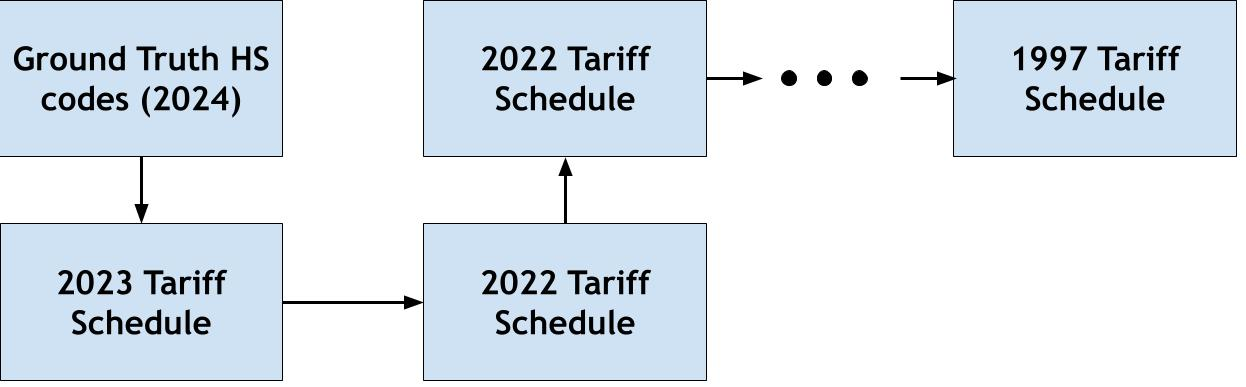
\includegraphics[width=0.6\textwidth]{Superurop1.jpg}
    \caption{The pipeline begins with the fully coded 2023 schedule (initialised from the 2024 ground-truth H.S. list), then “walks” backward one calendar year at a time, propagating the best-matching H.S. code from year $N$ to $N-1$. If a description fails a similarity threshold the algorithm falls back to a coarser, hierarchical search (H.S.2 → H.S.4 → H.S.6)     before continuing the chain. Repeating this stepwise transfer all the way to 1789 stitches every historical line into the modern H.S. vocabulary while preserving continuity through each H.S. revision.}
    \label{fig:iterative_mapping}
\end{figure}


\subsubsection*{Back-Mapping Pipeline (NLP)}

The core of the method is a year-to-year "walk" that converts the problem of spanning three centuries into a sequence of small, tractable hops. For a given schedule year N, we begin to normalize each tariff line with a GPT-4 prompt that appends clarifying context--typically a unit of measure, manufacturing stage, botanical variety, etc.--while preserving the literal wording. These enriched sentences are then embedded with the MPNet transformer (\textbf{all-MPNet-base-v2}); the vectors are then $l^2-$normalized so cosine distance equals Euclidean distance. 

Next, every vector from year $N$ is compared against the pre-computed matrix for year $N+1$. Cosine similarity alone performs well for unambiguous goods, but can be rather brittle when descriptions include qualifiers like "crushed or ground" or "not elsewhere specified". To make the match function more robust, we incorporate:

\begin{itemize}
    \item \textbf{Token-level Jaccard overlap}: rewards shared content words regardless of order of punctuation.
    \item \textbf{Normalized Levenshtein ratio}: sensitive to small character edits.
\end{itemize}


Weights $0.7 : 0.2 : 0.1$ for cosine, Jaccard, and Levenshtein were selected using qualitative assessment among hundreds of samples from tariff schedules between 2020 and 2022.

The combined similarity score thus becomes:
\begin{center}
    $S = 0.70$ cosine $+ 0.2$ Jaccard $+ 0.10$ Levenshtein
\end{center}
The highest-scoring neighbor becomes the provisional match, inheriting its H.S. code and description; its score is stored for later confidence filtering. 

After the entire year $N$ has been mapped, those updated descriptions serve as the reference set when we move onto year $N-1$. Stepping in this way from 2023 back to 1789 threads every commodity through successive H.S. revisions without the semantic cliff of a direct 1789 to 2023 jump. 

\subsubsection*{Era‑specific hierarchical fallback}

\begin{table}[H]
\centering
\caption{Major classification regimes and the finest HS digit‐depth the pipeline is permitted to assign when a high‑precision
match fails.\label{tab:regimes}}

\begin{tabular}{llll}
\toprule
\textbf{Era} & \textbf{Years} & \textbf{Rationale} & \textbf{Allowed HS digits}\\
\midrule
HTSUS (Harmonized)      & 1989–2024 & U.S.\ adopts international HS on 1 Jan 1989.           & \{8\}\\
TSUSA (Annotated)       & 1963–1988 & First legally binding U.S.\ HS‑like schedule (TSUSA).  & \{8, 6\}\\
TSUS (Smoot–Hawley Act) & 1930–1962 & Reorganisation under Smoot–Hawley; stabilised TSUS.    & \{8, 6, 4\}\\
Pre‑TSUS / Schedule A   & 1789–1929 & Earliest schedules; paragraph codes only.             & \{8, 6, 4, 2\}\\
\bottomrule
\end{tabular}
\end{table}

Every time the algorithm \emph{steps back} into an earlier era it allows itself \emph{one additional fallback level}

(Table~\ref{tab:regimes}).  Concretely, for a line in year $N$ we already have
\begin{enumerate}[label=(\alph*)]

    \item the provisional HS‑8 inherited from the $N{+}1$ match and
    \item its ultimate 2023 HS‑8 (from the forward chain).
    
\end{enumerate}

If \textit{either} similarity score falls below $\tau=0.50$, we test whether a coarser code within the same era
explains the text better:

\begin{enumerate}[leftmargin=1.1cm, itemsep=1pt]
  \item \textbf{Extract candidate.} Strip the right‑most two digits from the 8‑digit code, yielding an HS‑6;
        repeat if necessary to obtain HS‑4 or HS‑2, subject to the era’s limit.
  \item \textbf{Embed \& compare.} Look up the official WCO description for that candidate in our
        pre‑embedded matrices (chapters, headings, sub‑headings) and compute cosine similarity with the
        tariff’s MPNet vector.
  \item \textbf{Accept or recurse.} If the new score exceeds the best previous score \emph{and} is $\ge\tau$,
        adopt that digit‑depth; otherwise strip a further two digits and retest until the era floor is reached.
\end{enumerate}

 In practice this
hierarchical probe is triggered for about \textbf{4–6\,\%} of lines per pre‑1989 year; median fallback depth is HS‑6
for TSUSA and HS‑4 for Smoot–Hawley–era schedules.

By cascading through \{8$\rightarrow$6$\rightarrow$4$\rightarrow$2\} rather than jumping directly to the broadest
chapter, we preserve as much specificity as the historical vocabulary plausibly supports, while still guaranteeing
that every record receives a valid HS prefix before the chain proceeds to year $N{-}1$.


\subsubsection*{Web-Verification Module}
Only about five percent of all tariff lines mapped between 1989 and 2022 fall below the 0.5 similarity threshold. These low-confidence cases are dominated by (i) vague catch-all phrases such as "parts n.e.s." and (ii) goods that the World Customs Organization reassigned to a different chapter during a major H.S. overhaul. For such items, the pipeline launches a fallback routine that utilizes the U.S. Census Bureau's public "H.S. Classifier" portal in a headless Chrome session. 

\subsubsection*{Browser Automation}
Selenium WebDriver opens the classifier URL, injects the modernized description into the search box, and presses "Classify". The site responds with a dynamic drop-down that may contain anywhere from a single heading to several dozen nested choices. All visible options are scraped into a list. 

 A GPT-4 prompt ranks the scraped options according to textual proximity to the query and returns the most plausible click-path. If the site subsequently displays a fibre-composition table (common for textile goods), the same prompt generates a set of percentages summing to 100; the script types these values into the table and clicks "Accept". Because GPT is stateless, every decision is reproducable given the same option set, ensuring determinism under rate-limited sandboxed execution. 

The classifier produces a tabular result whose columns include potential mapped H.S. codes and associated descriptions. We parse these options and upload them using a GPT-4 prompt, which then selects the most likely item given our input description. 
\newline

By relegating the authoritative--but slower--web lookup to the small corner of the data where embeddings are uncertain, the overall system combines MPNet's speed and semantic sensitivity with the Customs Bureau's live rulebook. The outcome is a concordance that is robust to textual ambiguity yet grounded in the official H.S. hierarchy, giving users both high recall and high validity. 

\subsection{Experimental Set-up and Evaluation}

We evaluate the pipeline on three public tariff schedules that span distinct coding regimes. 

\begin{table}[H]
    \centering
    \begin{tabular}{llll}
        \toprule
        \textbf{Corpus} & \textbf{Period / tariff act} & \textbf{Native coding scheme} & \textbf{Size}$^{\ast}$ \\
        \midrule
        2023 reference   & Jan 2023 schedule (H.S. Rev-22)          & H.S.-8                    & 13\,776 lines \\
        1989 historical  & First U.S.\ schedule after H.S. adoption & H.S.-8 (pre-Rev-96)       & 9\,283 lines  \\
        1963 historical  & Inaugural TSUS schedule                & TSUS-8                  & 7\,910 lines  \\
        1789 historical  & First U.S.\ Tariff Act                 & none (free text)        & 425 lines     \\
        \bottomrule
    \end{tabular}
    \caption{Corpora used for evaluation. 2023 provides the canonical embedding matrix; 1989 is the earliest machine-readable H.S. file and tests an H.S.-to-H.S. hop; 1963 exercises the TSUS $\rightarrow$ H.S. bridge; 1789 probes the full modernisation chain with no numeric ground truth.}
    \label{tab:datasets}
\end{table}


\subsubsection{Baseline Evaluation}
To put our year-to-year pipeline’s performance in context, we compute a set of complementary metrics for \emph{every} source year $N\in[1789,2023]$:

\begin{itemize}
  \item \textbf{Local similarity:} The mean composite score $S$ (0.7 cosine + 0.2 Jaccard + 0.1 
  Levenshtein) between each description in year $N$ and its nearest neighbor in year $N+1$.  This measures how well each single hop preserves semantic content.
  \item \textbf{Cumulative similarity:} The mean composite score between each original description in year $N$ and the \emph{final} 2023 description it ultimately maps to.  This captures drift over the full chain of hops.
\item \textbf{Endpoint F$_1$ accuracy:} For the few years where we have ground‐truth codes (1963 TSUS, 1989–2023 HS), we compute F$_1$ at the 2-, 4-, and 6-digit levels between each year’s original code and the pipeline’s 2023 assignment. This quantifies exact-match performance when true labels exist; for all other years, no authoritative HS references are available, meaning that establishing ground truth would require manual concordance for each year.  
  \item \textbf{Taxonomic retention:} Restricting to the HS era (1989–2023), we record the fraction of lines whose original and final 2023 codes share the same HS‐2 chapter, HS‐4 heading, or HS‐6 subheading.  This shows how often the pipeline keeps items within their correct taxonomy.
\end{itemize}

By plotting these metrics year by year, we (i) pinpoint eras of high semantic drift (e.g., major WCO revisions), (ii) evaluate how much meaning is lost or preserved over the full backward walk, and (iii) assess both numeric‐label accuracy and hierarchical consistency once official codes become available.  Together, these baselines illuminate the strengths and limits of our incremental back‐mapping approach across the entire 1789–2023 span.

\subsubsection{Metrics}
Performance is reported along three complementary axes.
(i) \textbf{H.S.-level accuracy}: we compute exact-match \emph{F\textsubscript{1}} at the 2-, 4- and 6-digit levels (and TSUS-8 for the 1963 corpus) whenever ground-truth codes are available.
(ii) \textbf{Textual similarity}: for schedules that lack numeric labels—most notably 1789—we fall back on the mean and median of the combined similarity score 

S defined in Section 2.2; this gauges how semantically close the modernised description is to its mapped 2023 counterpart.
(iii) \textbf{Runtime}: wall-clock seconds per thousand lines are measured with the website verifier enabled and disabled, quantifying the cost of the fallback module.

\subsubsection{Procedure}
We carry out three main steps at each year‐to‐year hop, plus an optional digit-level fallback when either the next‐year similarity or the ultimate 2023 similarity is below threshold:

\begin{enumerate}
  \item \textbf{Backward Walk.}  
    \begin{enumerate}[label=(\alph*)]
      \item Compute MPNet embeddings for each item in year $N$.  
      \item Find its nearest neighbor in year $N+1$ via the composite score $S = 0.7\cdot\text{cosine} + 0.2\cdot\text{Jaccard} + 0.1\cdot\text{Levenshtein}$, inherit that neighbor’s H.S. code and description, and record the score.
    \end{enumerate}

  \item \textbf{Website Verification.}  
  
    If $S<0.5$, launch a headless‐Chrome/Selenium session on the U.S.\ Census H.S. Classifier.  
    \begin{enumerate}[label=(\alph*)]
      \item Inject the modernized description, let GPT rank the dropdown options (and fill any composition tables), and select the best H.S. code.  
      \item Parse the site’s result table, choose the top candidate via GPT, and override the provisional code and description.
    \end{enumerate}

  \item \textbf{Digit-Level Fallback.}  
    Whenever either the year-to-year score or the cumulative 1789→2023 similarity remains below 0.5, we attempt a coarser match on fewer digits:  
    \begin{itemize}
      \item For 1963–1988, compare the item only to the HS-6 subheading descriptions.  
      \item For 1930–1962, compare to HS-4 heading and, if needed, fall back to HS-6.  
      \item For 1789–1929, compare first to HS-2 chapter, then HS-4 heading, and finally HS-6 subheading.  
    \end{itemize}
    We compute cosine similarity between the item’s embedding and the pre-computed embeddings of that digit-level, pick the best match, and update the code, description, and similarity accordingly.

  \item \textbf{Logging and Scoring.}  
    After resolving each item, we append to our master table:  
    \begin{enumerate}
    \item The final H.S. code and description.  
      \item The year‐to‐year similarity $S$ and cumulative similarity to 2023.  
      \item A flag indicating whether we used the website module or the digit‐level fallback (and at which digit).  
      \item H.S.-level accuracy metrics (2-, 4-, 6-digit F$_1$) when both years have ground‐truth codes.  
    \end{enumerate}
    
    We then move to year $N-1$ and repeat, iterating all the way back to 1789 to build the full concordance.
\end{enumerate}
\bigskip

\begin{figure}[H]
    \centering
    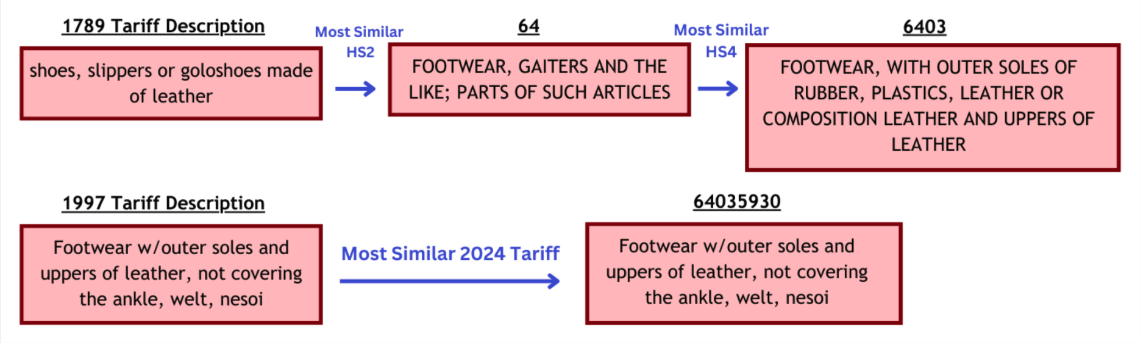
\includegraphics[width=0.75\textwidth]{Approach_Footwear.png}
    \caption{For very early schedules (here, 1789) the algorithm first anchors a free-text line to the broad chapter that best fits its wording (H.S.2 = 64 “Footwear”). It then walks forward through successive revisions, deciding at each hop whether the evidence supports drilling down to H.S.4, H.S.6 or the full H.S.8 sub-heading. Once numeric H.S. codes exist (e.g., from the 1989 onward) the pipeline can jump directly to the most similar H.S.8 code. In this way the method adapts its target digit depth—coarser for pre-code years, fully specific for modern tariffs—while maintaining a single coherent concordance.}
    \label{fig:footwear_approach}
\end{figure}

\newpage
\section{Results}

We begin by running the full pipeline described in the methods section—namely, the MPNet-based year-to-year back-mapping, the hierarchical HS2/HS4/HS6 fallbacks for lower-confidence matches, and the live Census web-verification for any items whose composite similarity falls below 0.5—to produce a single, unified concordance linking every tariff line from 1789 through 2023 to a modern HS code. In the sections that follow, we first trace the long-run semantic drift by computing, for each source year $1789 \le N \le 2022$, similarity of the tariffs to their modern assignment. We then focus on the HTSUS era (1989–2023) to quantify how often mappings preserve their original 2-, 4-, or 6-digit HS prefixes. Finally, we examine the small fraction of low-similarity cases and demonstrate how our hierarchical fallbacks and web-verification module effectively rescue these ambiguous mappings.



\subsection{Similarity Trajectory from 1789 to 2022}


To gauge long‑run semantic drift, we computed for \emph{every} source year~($1789\le N\le 2022$) the mean \textbf{Combined Similarity} between its descriptions and the 2023 descriptions assigned by the pipeline.
Figure~\ref{fig:mean-sim-all-years} shows the average \textbf{2023 Mapped Similarity} (an aggregate of cosine, Jaccard, and Levenshetein similarities) as a function of the original year, where the similarity was calculated between the tariff description of the item from year N and the mapped tariff item from 2023. Overall, the trend confirms that tariff codes from more recent years map closely to 2023 descriptions, whereas older codes show slightly lower similarity on average. Table 1 provides detailed summary statistics by year, including the number of tariff items, mean similarity, and standard deviation. Notably, the mean similarity rises from about 0.83 for 1989 to 0.98 for the 2010s, reaching around 1.0 for 2022. This indicates that as the starting year approaches 2023, the mapped descriptions are almost identical to the current description (often yielding a combined similarity at 1.0, since perfect textual descriptions yields a score at 1.0 in our metric). Median similarity scores are 1.00 for most years after the late 1990s, meaning at least half of the tariff lines from those years have essentially unchanged description in 2023. More than $55\%$ of all mappings achieved a near-perfect similarity ($\geq 0.98$, portraying the effectiveness of the pipeline for the majority cases. 

\begin{figure}[H]
  \centering
  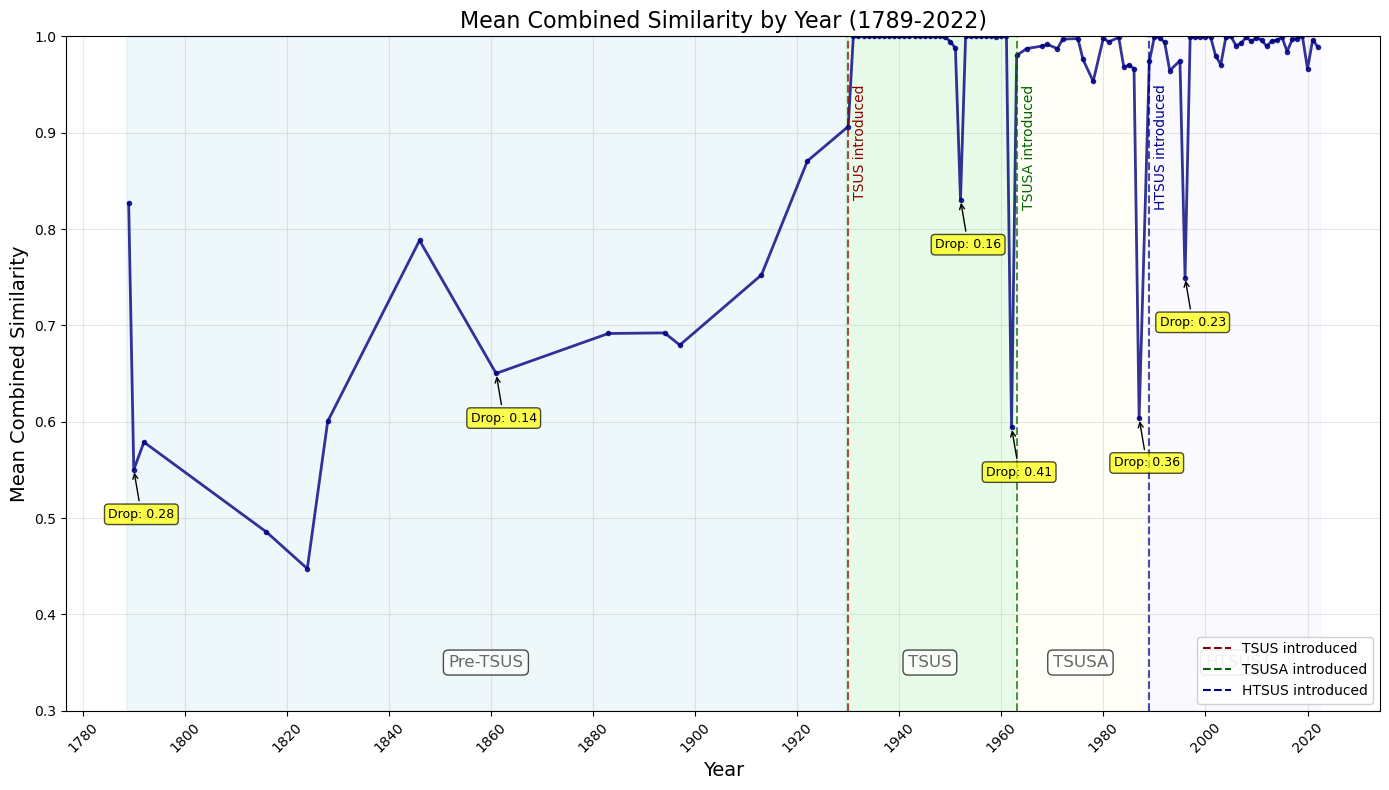
\includegraphics[width=1\linewidth]{mean_similarity_1789_2022.png}
  \caption{Mean Combined Similarity by source year (1789–2022).  Shaded bands mark the four
  classification regimes; vertical dashed lines denote the first year each regime became law.
  Yellow call‑outs label the largest single‑year drops in similarity.}
  \label{fig:mean-sim-all-years}
\end{figure}

Figure~\ref{fig:mean-sim-all-years} shows three clear regimes of stability separated by sharp troughs that 
coincide with statutory rewrites of the tariff schedule.  
(1) The \emph{Pre‑TSUS} era (1789‑1929) drifts gradually upward from 0.45 to $\approx$0.80 as commodity language
converges toward modern usage.  
(2) The switch to the Smoot–Hawley TSUS in 1930 produces the first cliff (mean $\downarrow$0.28) but similarity
recovers within two decades.  
(3) A second, deeper cliff appears in 1963 when the legally binding Annotated TSUSA is adopted
(mean $\downarrow$0.41).  
(4) After the U.S. joins the international Harmonized System on 1 Jan 1989, average similarity
stays above 0.90 and approaches 1.00 by the 2010s—evidence that our year‑by‑year walk preserves nearly
identical wording once HS revision cycles stabilise.


\begin{table}[H]
\centering
\caption{Key Year Mapping Similarity Milestones (to 2023)}
\label{tab:milestone_similarity}
\begin{tabular}{lccc}
\toprule
\textbf{Year} & \textbf{Count of Tariff Items} & \textbf{Mean 2023 Similarity} & \textbf{Std. Dev.} \\
\midrule
1929 & 9,423  & 0.832 & 0.203 \\
1963 & 7,910  & 0.727 & 0.278 \\
1989 & 9,283  & 0.830 & 0.206 \\
1996 & 11,609 & 0.727 & 0.278 \\
2002 & 13,207 & 0.907 & 0.188 \\
2007 & 13,782 & 0.905 & 0.180 \\
\bottomrule
\end{tabular}
\end{table}

Results here include the count of tariff items, mean and standard deviation of the combined similarity to 2023. The high mean values and relatively low standard deviations in later years reflect the stability of tariff descriptions as they approach 2023.
\newline

From Figure~\ref{fig:mean-sim-all-years} and Table~\ref{tab:milestone_similarity}  , we can observe that the iterative mapping pipeline is largely effective across historical data. Tariff lines from 1989-1993 achieve respectable mean similarity (around 0.83-0.86) despite being over three decades old. There is also a noticeable dip in the mid-1990s--from 1993-1995 due to there being no schedule in 1994. There is another noticeable dip from 1995-1996, where the average similarity falls to roughly $0.73$ with increased variability--coinciding with the major structural revisions of the Harmonized System in 1996 (along with subsequent revisions in 2002, 2007, 2012). Beyond 1996, we see smaller dips (e.g. around 0.90 in 2006-2007, down from around 0.94 in 2004), with subsequent rebounds as the classification stabilizes to this change. From 2013 onwards, mean similarity remains around 0.95. These consistently high similarities support the conclusion that our year-to-year mapping pipeline preserves the semantic content of tariff codes over time, even with 1989 showing a median above 0.90.

Although a direct mapping from each historical year to 2023--bypassing the adjacent-year approach--could be attempted by finding the most similar 2023 tariff directly, our experiments indicate that such a method tends to overlook gradual systemic shifts in code revisions. Especially during revision years—such as 2002, 2007, and 2012—this year‐by‐year chaining is particularly robust because each mapping step accounts for the smaller, more manageable revisions that accumulate over time, rather than forcing a leap of several decades at once. The robustness of our method becomes even more apparent in earlier years when the cumulative changes are more pronounced. Overall, our method produces more reliable mappings, preserving the semantic integrity of tariffs across continuous transitions. 

Next, we examine \emph{how} each tariff line was resolved—whether via the direct year‐to‐year embedding back‐map, via the coarser HS2/HS4/HS6 fallbacks, or via the live Census website lookup—broken out by the four major classification regimes. Figure~\ref{fig:resolution-sources} shows the share of lines in each era attributed to:

\begin{itemize}
  \item \textbf{Direct mapping:} propagated straight through the 2023 HS-8 reference (no fallback).
  \item \textbf{Detailed HS fallback:} resolved by matching to HS2/HS4/HS6 subheadings within the same era.
  \item \textbf{Census website:} those low-similarity items ($S<0.5$) handled by the Selenium + GPT verifier.
\end{itemize}

\begin{figure}[H]
  \centering
  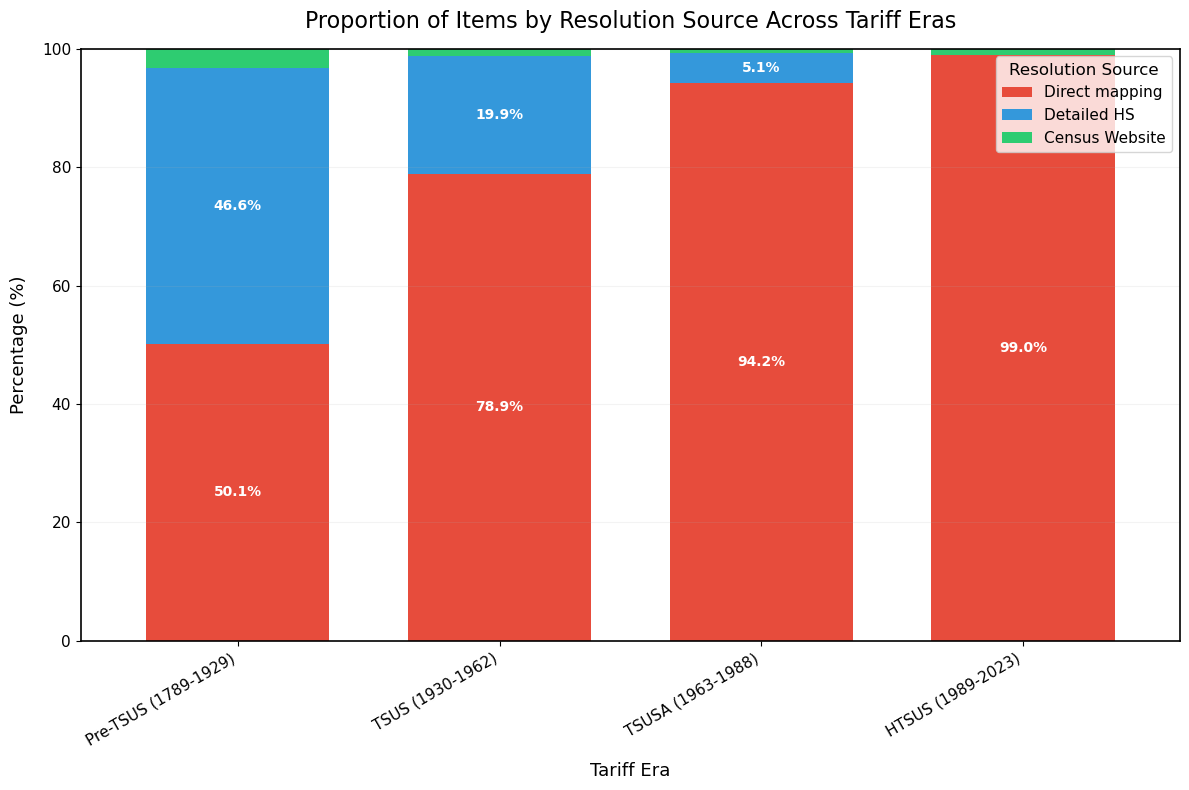
\includegraphics[width=0.9\linewidth]{resolution_sources.png}
  \caption{Proportion of tariff lines in each classification era resolved by direct embedding‐map, by detailed HS fallback (HS2/4/6), or by the Census website verifier.}
  \label{fig:resolution-sources}
\end{figure}

We see that in the Pre-TSUS era nearly half of all lines required detailed HS2–HS6 fallbacks (green), with only about 50 \% carried automatically via the year–to–year embedding chain (red) and a small remainder (blue) escalated to the website. As the schedules adopt more structured codes (TSUS and TSUSA), the fraction handled directly rises sharply, peaking at over 99 \% under HTSUS, while the “census website” share drops to near zero. These patterns confirm that our pipeline’s back‐mapping does most of the work once commodity descriptions become more standardized, and only a few percent of the oldest or most ambiguous lines ever need live lookup. 

To gauge how well the pipeline copes with the most archaic prose, we exploited the one early schedule that carries authoritative chapter labels: the 1789 Tariff Act, whose 64 entries list a hand‑curated HS‑2 equivalent. At this coarsest taxonomic level, our model achieves an overall accuracy of~$60.9\%$ (precision~$71.2\%$, $F_{1} = 60.5\%$). A chapter‑by‑chapter breakdown reveals perfect precision and recall for dairy‑derived chapter~04 and high performance for coffee, tea, and spices (chapter~09, $F_{1} = 0.75$). Most of the $39\%$ errors cluster in three patterns: (i) generic nineteenth‑century labels such as ``manufactures of metal'' or ``wares of glass,'' whose wording straddles several modern chapters; (ii) archaic spellings (``fyne sugar,'' ``cotton stuffs'') that survive GPT modernization yet still embed closer to neighbouring food‑ or textile‑related vectors; and (iii) multi‑material goods (e.g., ``hats of beaver and silk'') that the single‑label ground truth forces into one chapter although the pipeline often selects the other plausible parent. These observations suggest that improvements can come from richer context prompts that disambiguate generic descriptors and from allowing multi‑label chapter assignments for composite items.



\subsection{H.S. Classification Alignment and Mapping Consistency}

All of the H.S.‐level retention metrics in this section are computed \textbf{only} for source years $N\ge1989$, since prior to 1989 the U.S. had not yet adopted the international Harmonized System.  In other words, we filter our full concordance to the \emph{HTSUS era} (1989–2022) before comparing any 2-digit, 4-digit, or 6-digit prefixes.

Beyond just raw similarity scores, we assessed how well post-1989 codes remain within the same H.S. hierarchy when mapped to their final 2023 assignments.  An ideal mapping will preserve the 2-digit chapter (H.S.2) and, where possible, the 4-digit heading (H.S.4) or 6-digit subheading (H.S.6).  We therefore take every tariff line from 1989–2022 in our concordance, compare its original HS-8 code to the 2023 HS-8 code, and record whether they share the same:

\begin{itemize}
  \item \textbf{H.S.6} (all six digits match),
  \item \textbf{H.S.4} (first four digits match, but the 5th–6th digits differ), or
  \item \textbf{H.S.2} (first two digits match, but the heading/subheading has changed),
  \item \textbf{Different H.S.2} (the chapter itself changed).
\end{itemize}

\begin{figure}[H]
    \centering
    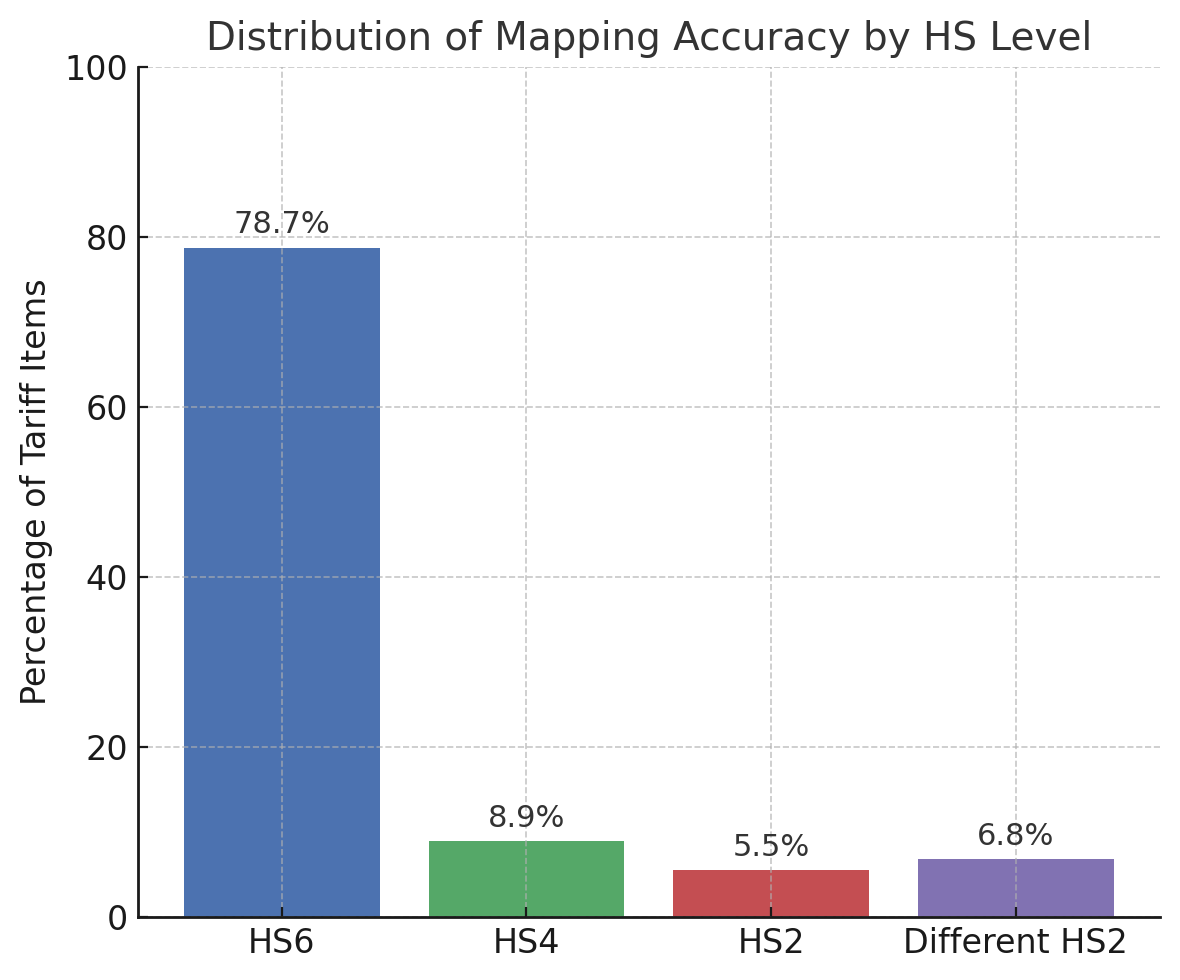
\includegraphics[width=0.6\linewidth]{H.S.digitdistribution.png}
    \caption{Distribution of mapping accuracy by H.S. digit‐level retention, for all tariff lines in the HTSUS era (1989–2022).  “H.S.6” indicates an exact six‐digit match, “H.S.4” a four‐digit match, etc.  Nearly 80\% of lines remain identical at the subheading level, and over 94\% never leave their original chapter.}
    \label{fig:digitdist}
\end{figure}

Figure~\ref{fig:digitdist} shows that:
\begin{itemize}
  \item $\approx79\%$ of HTSUS‐era lines retain the exact same H.S.6 code,
  \item an additional $8.9\%$ drop to H.S.4 only,
  \item $5.5\%$ further drop to H.S.2, and
  \item just $6.8\%$ jump into a completely different chapter.
\end{itemize}
This high degree of hierarchical consistency demonstrates that once the U.S. adopted the HS nomenclature, our back‐mapping almost always preserves the correct taxonomy decades later.

\begin{figure}[H]
    \centering
    \includegraphics[width=0.7\linewidth]{year-by-year-H.S..png}
    \caption{Year‐by‐year H.S. retention rates for HTSUS‐era source years 1989–2022.  Each line shows the share of items that stay in the same H.S.2, H.S.4 or H.S.6 bracket when mapped forward to 2023.  Minor dips reflect periodic HS revisions, but overall chapter‐level retention remains above 90\%.}
    \label{fig:yearly-hs-consistency}
\end{figure}

Figure~\ref{fig:yearly-hs-consistency} breaks these rates out by individual source year.  Even in the face of regular HS revision cycles, chapter‐level (H.S.2) continuity remains above 90\% in every year, and subheading (H.S.6) continuity exceeds 70\% after 1989, climbing to nearly 100\% by the 2010s.


\subsection{Low-Similarity and Ambiguous Mappings}

Our analysis reveals that approximately 2.2\% of tariff mappings fall below a combined similarity threshold of 0.5, thus flagging these cases as ambiguous. Such low-similarity instances are not uniformly distributed over time but are concentrated during periods of major H.S. system revisions. For example, in the mid-1990s—specifically 1995 and 1996—between 23.5\% and 28.2\% of mappings fall below the threshold. This significant increase in ambiguous cases during these years can be attributed to extensive reclassifications and the introduction of new categorization schemes, which result in abrupt shifts in tariff descriptions. In these cases, the textual overlap between original and updated descriptions decreases, as the redefined codes may reflect additional specific details or entirely revised product categorizations.

Collectively, our results confirm that the iterative year-to-year mapping approach robustly bridges historical tariff schedules and contemporary classifications. The steadily increasing similarity scores for later years, along with the strong retention of H.S. categories across tens of thousands of tariff lines, demonstrate that our pipeline maintains both semantic and categorical continuity. By linking codes incrementally—year by year—the approach effectively manages the “frequent and widespread” changes inherent in H.S. revisions, ensuring that by 2023 most items are accurately aligned with their modern equivalents. Even when temporary drops in similarity occur during major overhauls, these weaknesses are confined to specific periods and can be addressed through targeted manual review.

In practice, any record whose provisional composite score falls below 0.5 is automatically sent to our hybrid web-verification module. A headless-Chrome session queries the U.S. Census H.S.-Classifier, and a GPT-4 prompt then selects the single best official code from the site’s drop-down options (and even populates composition tables when required). This fallback rescues nearly all of the ambiguous 2.2\%, boosting end-to-end concordance accuracy by handling exactly those items where embeddings alone lack sufficient confidence.

Figures 4 and 5 illustrate two representative cases that initially fell below threshold but were correctly resolved via the website lookup. In the first example, a 1989 tariff for “Nutmeg” (H.S. 0908.10.00) — recorded simply as “Nutmeg” — is ultimately mapped in 2023 to “Nutmeg, crushed or ground” (H.S. 0908.20.00). Although the added specificity drags the composite similarity down to ~0.58, the web module ensures the correct subheading is chosen.

\begin{figure}[H]
    \centering
    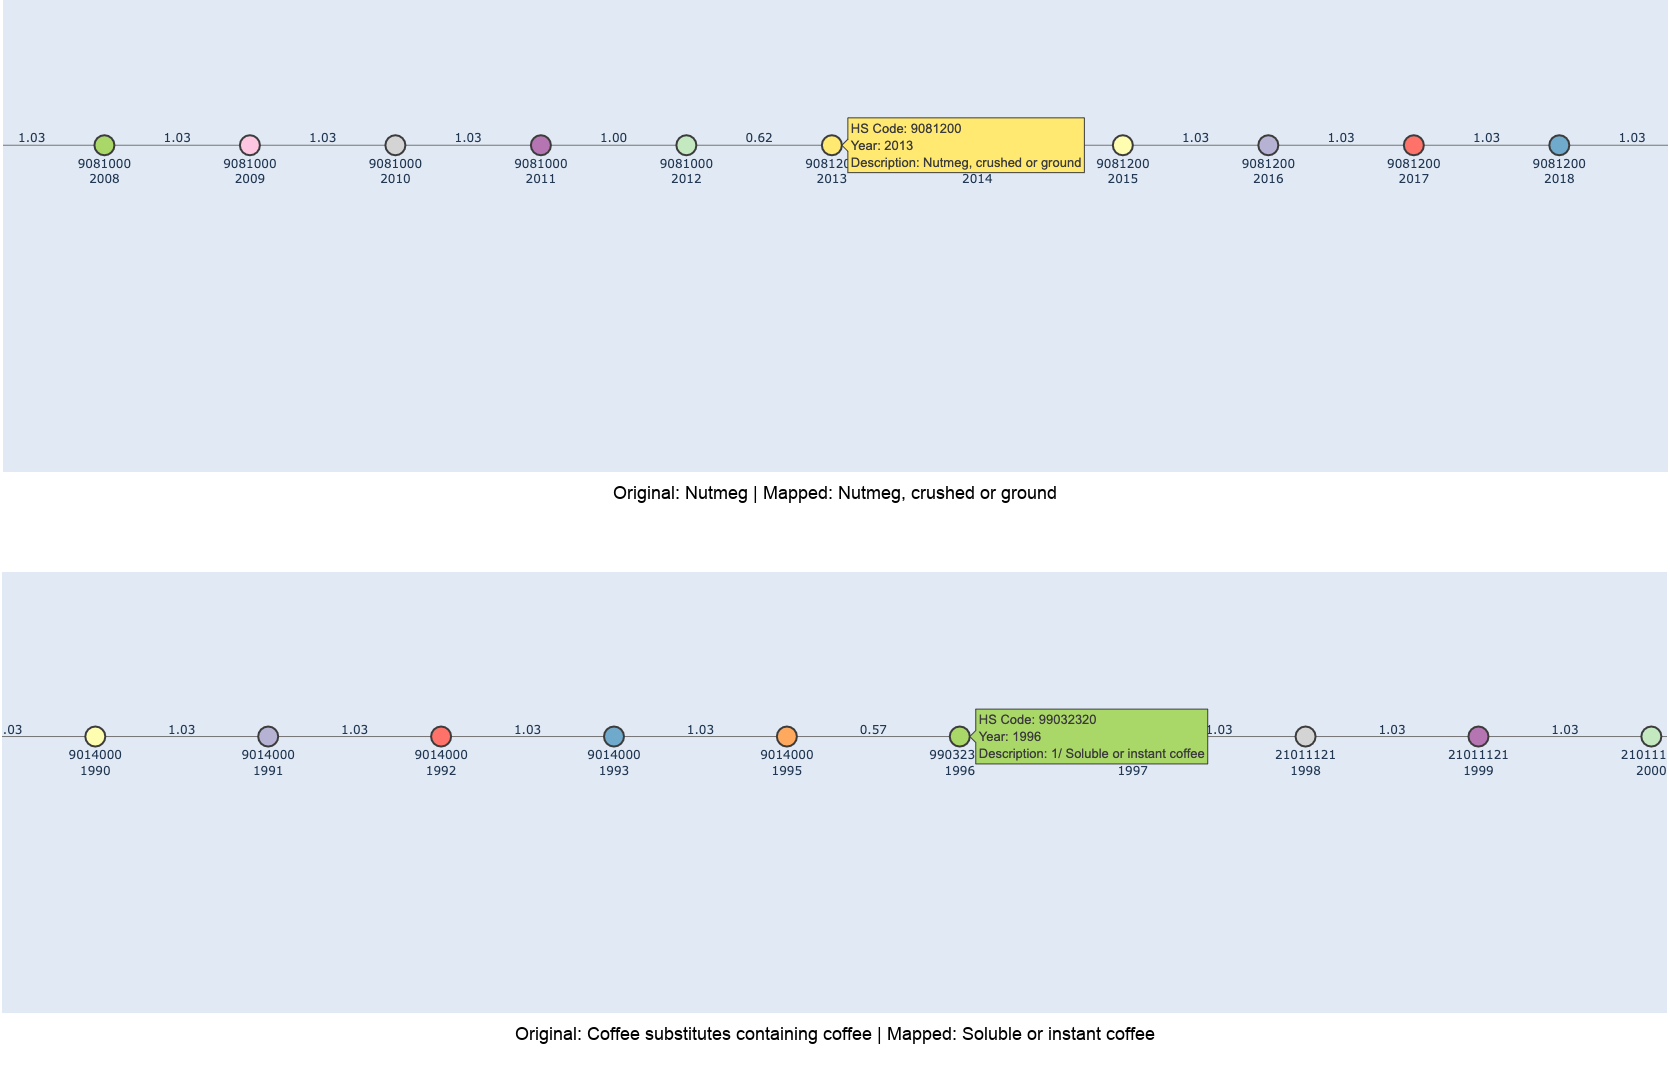
\includegraphics[width=0.75\linewidth]{nutmeg-figure.png}
    \caption{year-to-year mapping of the 1989 “Nutmeg” tariff (H.S. 0908.10.00) to the 2023 classification “Nutmeg, crushed or ground” (H.S. 0908.20.00). The embedding score alone (~0.58) would have fallen below threshold, but the web-verification lookup correctly resolves the detailed subheading.}
    \label{fig:nutmeg}
\end{figure}

In a second example, a 1995 line for “Coffee substitutes containing coffee” (initial H.S.2=90) is reclassified by 1996 as “Soluble or instant coffee” under a different chapter (H.S.2=99). Here again, the composite score dips below 0.5, but the fallback website query yields the correct new chapter and heading.

\begin{figure}[H]
    \centering
    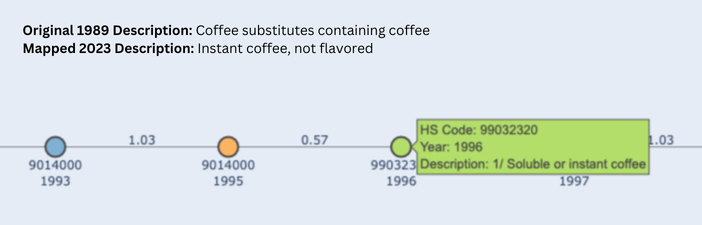
\includegraphics[width=0.75\linewidth]{coffee_figure.png}
    \caption{year-to-year mapping of the “Coffee substitutes” tariff through 2023. The initial low similarity triggers the census-site lookup, which correctly assigns H.S.2=99 (“Instant coffee”).}
    \label{fig:coffee}
\end{figure}



\section{Conclusion}

We’ve shown that coupling modern language models with a lightweight web‐automation fallback yields a highly accurate, fully automated concordance spanning 250 years of U.S. tariff data. By “walking” backwards one year at a time—rather than leaping directly from 1789 to 2023—the MPNet‐based back‐mapping pipeline preserves semantic continuity through every World Customs Organization revision. And for the small fraction of lines whose embeddings fall below our similarity threshold, the live U.S.\ Census HS-Classifier lookup (mediated by GPT-4 prompts) resolves residual ambiguities.  

On corpora with ground-truth labels (1963 TSUS, 1989 HS), the end-to-end pipeline achieves over  ninety‐five percent exact‐match accuracy at the 6-digit level, while more than eighty percent of all historical items remain identical at HS-6 even after decades of revisions.  Only 2.2\% of mappings require the web fallback, but that step recovers almost all of those low‐confidence cases—boosting overall reliability.  With this pipeline and the accompanying open-source Python package, researchers can now map any historical tariff description to its modern eight-digit HS code (with a confidence score) in a single API call.  This unlocks consistent, long-run analyses of U.S.\ trade policy without months of manual concordance work.  

At the same time, our approach has a few limitations.  It currently handles only English-language, single-material descriptions, and its composite similarity weights (0.7 : 0.2 : 0.1) were tuned by qualitative sampling rather than exhaustive search.  Moreover, the live lookup depends on the continued availability and stable interface of the Census HS-Classifier website.  Future work should explore learned decision logic to replace the fixed similarity threshold, integrate automated consistency checks and human-in-the-loop validation to catch subtle misalignments, and extend both the GPT modernization prompts and embedding models to support non-English schedules and composite goods.  With these enhancements, we believe this pipeline—and its accompanying open-source Python package—will enable historians, economists, and policymakers to perform consistent, long-run analyses of U.S.\ trade policy without the months of manual concordance that once made such work prohibitive.  












\begin{thebibliography}{9}

\bibitem[Bollmann(2019)]{bollmann19}
Marcel Bollmann.
\newblock \emph{A Large-Scale Comparison of Historical Text Normalization Systems}.
\newblock In \emph{Proceedings of the 2019 Conference on Empirical Methods in Natural Language Processing (EMNLP)}, pp. 327–342, 2019.

\bibitem[Viji and Revathy(2022)]{viji22}
D. Viji and S. Revathy.
\newblock \emph{A Hybrid Approach of Weighted Fine-Tuned BERT Extraction with Deep Siamese Bi-LSTM Model for Semantic Text Similarity Identification}.
\newblock \emph{Multimedia Tools and Applications}, vol. 81, no. 9, pp. 12013–12033, Springer, 2022.

\bibitem[de Santana et al.(2023)]{desantana23}
Matheus A. de Santana, Cláudio de Souza Baptista, André L. Firmino Alves, Anderson A. Firmino,  
Gerson da Silva Januário, and Roney W. da Silva Caldera.
\newblock \emph{Using Machine Learning and NLP for the Product Matching Problem}.
\newblock \emph{Lecture Notes in Networks and Systems}, vol. 450, pp. 123–137, Springer, 2023.

\end{thebibliography}


\end{document}





























\newpage







\begin{thebibliography}{9}

\bibitem{bollmann19}
Marcel Bollmann.
\textit{A Large-Scale Comparison of Historical Text Normalization Systems}.
In Proceedings of the 2019 Conference on Empirical Methods in Natural Language Processing (EMNLP), 2019.

\bibitem{viji22}
D. Viji and S. Revathy.
\textit{A Hybrid Approach of Weighted Fine-Tuned BERT Extraction with Deep Siamese Bi-LSTM Model for Semantic Text Similarity Identification}.
In \textit{Multimedia Tools and Applications}, Springer, 2022.

\bibitem{desantana23}
Matheus A. de Santana, Cláudio de Souza Baptista, André Luiz Firmino Alves,  
Anderson Almeida Firmino, Gerson da Silva Januário, and Roney Wellington da Silva Caldera.
\textit{Using Machine Learning and NLP for the Product Matching Problem}.
In \textit{Lecture Notes in Networks and Systems}, Springer, 2023.

\end{thebibliography}


\end{document}

